% !TEX root = main.tex

\clearpage
\section{Decay-time Resolution}
\label{sec:Resolution}

The observed oscillation of B mesons is prone to dilution, if the detector resolution is of similar magnitude as the oscillation period. 
In the \Bs system, considering that the measured oscillation frequency of the \Bs \cite{PDG2014} and the average LHCb detector resolution \cite{LHCb-DP-2014-002} are both 
$\mathcal{O}(50 \fs^{-1})$, this is the case.
Therefore, it is crucial to correctly describe the decay time resolution in order to avoid a bias on the measurement of time dependent CP violation. 
Since the time resolution depends on the particular event, especially the decay time itself, 
the sensitivity on $\gamma$ can be significantly improved 
by using an event dependent resolution model rather than an average resolution.
For this purpose, we use the per-event decay time error that is estimated %for each event $i$, is 
based on the
uncertainty obtained from the global kinematic fit of the momenta and vertex positions (DTF) with additional constraints on the PV position and the $D_s$ mass.
In order to apply it correctly, it has to be calibrated.
The raw decay time error distributions 
for $\Bs\to\Ds\pion\pion\pion$ signal candidates
are shown in Figure \ref{fig:Bs_DTFERR_Comp} for Run-I and Run-II data.
Significant deviations between the two different data taking periods are observed
due to the increase in center of mass energy from Run-I to Run-II, as well as (among others) new tunings in the pattern and vertex reconstruction.
The decay time error calibration is consequently performed separately for both data taking periods.

For Run-I data, we use the calibration from the closely related $\Bs\to\Ds\kaon$ analysis which was performed on a data sample of prompt-$D_s$ candidates combined with a random pion track from the PV. We verify the portability to our decay channel on MC.

For Run-II data, a new lifetime unbiased stripping line (LTUB) has been implemented which selects prompt-$D_s$ candidates combined with random $K\pi\pi$ tracks from the PV.



%%Significant deviations can be observed in the shape and mean of those two distributions for $\Bs\to\Ds\pion\pion\pion$ signal candidates shown in Figure \ref{fig:Bs_DTFERR_Comp}.
%It can be observed that the decay time error distribution for signal candidates from Run II is significantly broader and shifted to slightly higher values.
%Due to the discrepancies between the distributions of the decay time error $\sigma_{r}$ for Run-I and Run-II data, the decay time resolution studies have to be performed separately.

\begin{figure}[h]
\centering
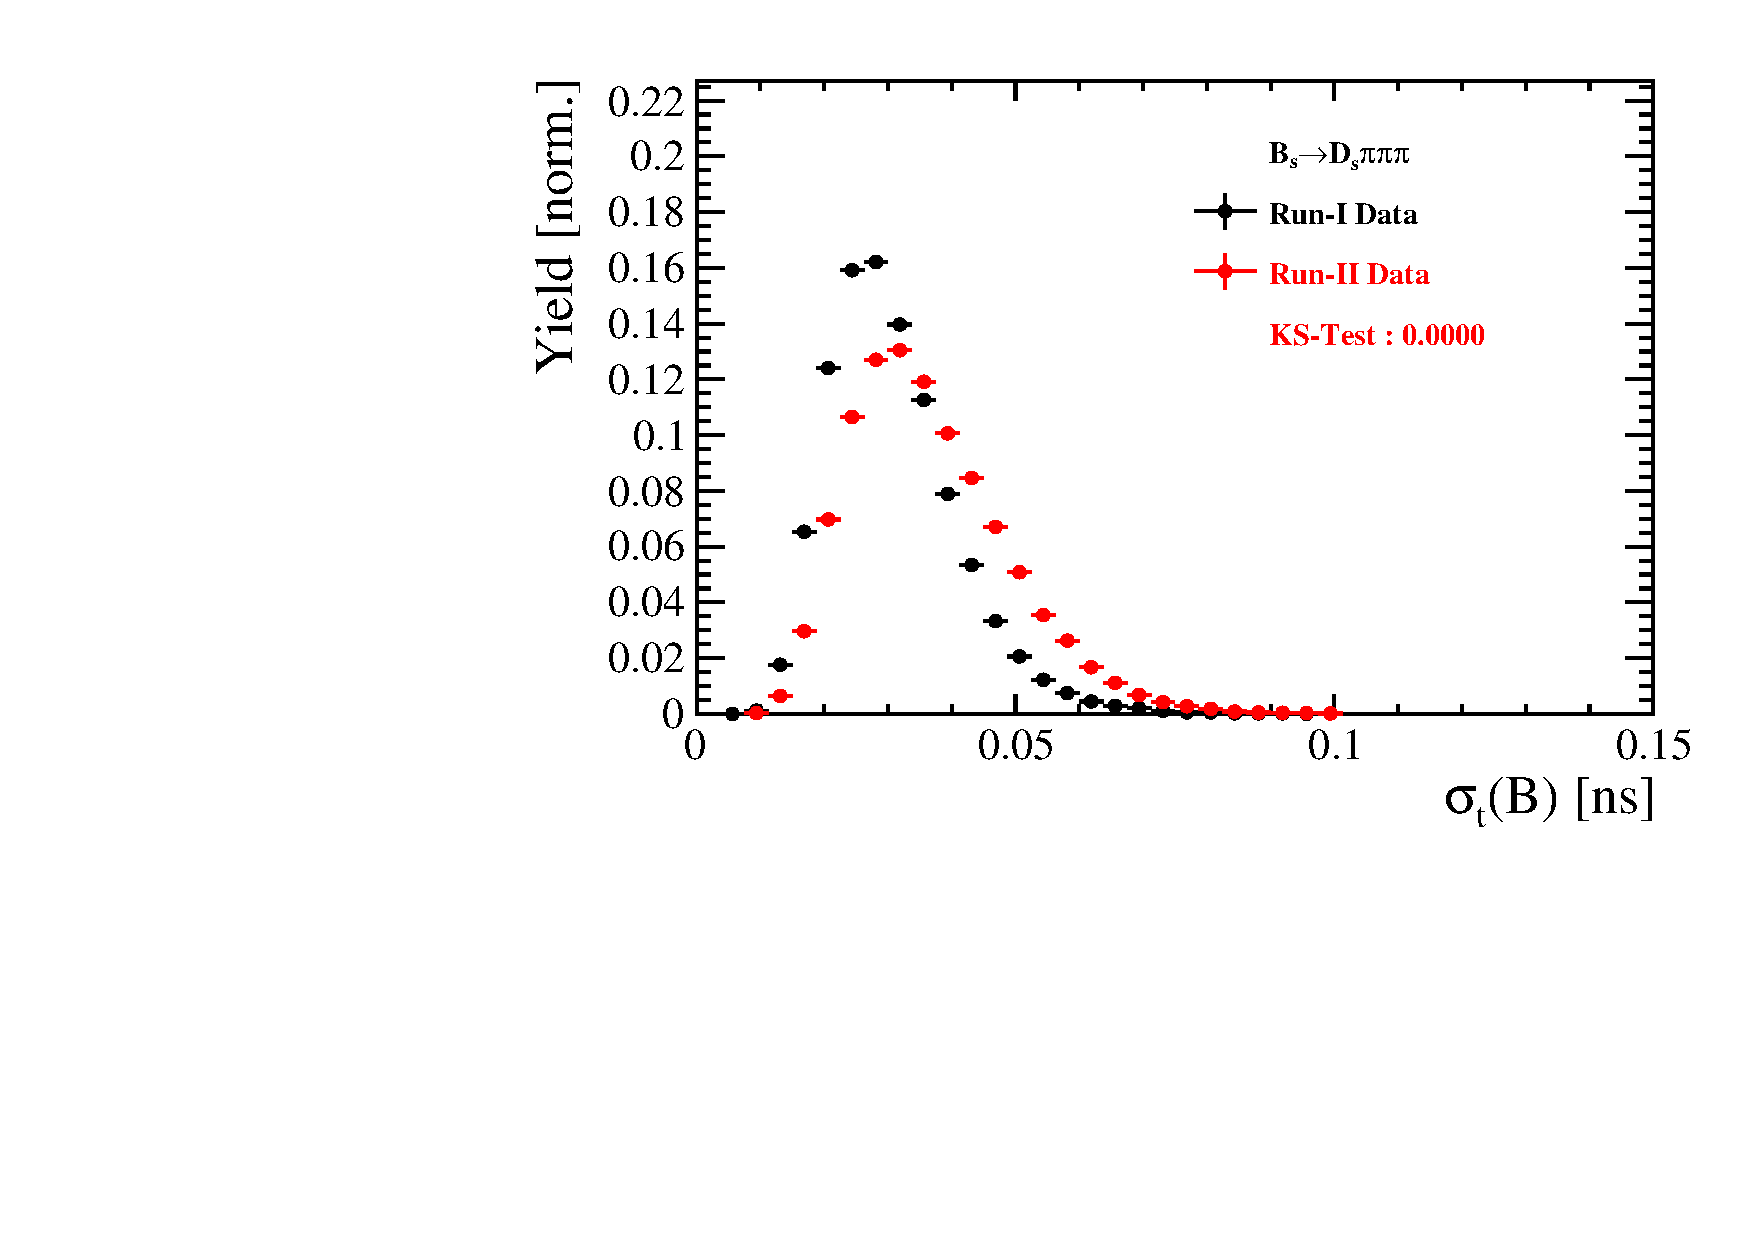
\includegraphics[height=!,width=0.7\textwidth]{figs/dataVsMC/run1vs2_norm/Ds2all_Bs_DTF_TAUERR.pdf}
\caption{Distribution of the decay time error for $\Bs\to\Ds\pion\pion\pion$ signal candidates for Run-I (black) and Run-II (red) data (sWeighted).}
\label{fig:Bs_DTFERR_Comp}
\end{figure}

%In the presented analysis, we assume a gaussian resolution function with different widths for each event. 
%This gives rise to a per-event decay time error $\sigma_{t}$, which is computed separately for every event along with the proper time $t$, by the decay time fitter. 
%Furthermore, the per-event decay time error $\sigma_{t}$ is usualy underestimated by the decay time fitter, 
%making it necessary to derive a scaling function, which matches the per-event error to the actually measured decay time resolution. \newline
%Due to the lack of a decay time unbiased sample of real $\Bs\to\Ds\kaon\pion\pion$ decays, this analysis relies on simulation to describe the time resolution. 
%The obtained results will be compared to those found in the closely related $\Bs\to\Ds\kaon$ analysis and systematic uncertainties will be assigned conservatively.
%In the following, we investigate the Run1 and Run2 MC samples to find the proper decay time resolution in bins of the per-event decay time erros and derive a scaling function from that.      

\clearpage
\subsection{Calibration for Run-I data} 

For simulated $\Bs\to\Ds\kaon\pion\pion$ events, the
spread of the 
differences between reconstructed decay time and true decay time,
$\Delta t = t - t_{true}$, 
is a direct measure of the decay time resolution.
The sum of two Gaussian pdfs with common mean but different widths is used to fit the distribution of the decay time difference $\Delta t$
%One Gaussian function is relatively narrow and describes the decay time of the majority of candidates in each bin, 
%while the other, broader Gaussian function describes candidates where the measure decay time differs considerably from $\tau_{true}$. 
%Those contributions are shifted to the tails of the distribution. 
%From the two Gaussian functions, the combined, effective width $\sigma_{eff}$ is quoted as decay time resolution in each bin. 
as shown in Fig.~\ref{fig:scaleFactorMC}. 
%For the combination of the two separate widths $\sigma_{1}$ and $\sigma_{2}$, a method which takes the damping effect of the finite time resolution on the CP observables into account, is used.
The effective damping of the CP amplitudes due to the finite time resolution is described by the dilution $\mathcal{D}$.
%, which can take values between 1 and 0. 
In the case of infinite precision, there would be no damping and therefore  $\mathcal{D} = 1$ would hold, 
while for a resolution that is much larger than the $\Bs$ oscillation frequency, $\mathcal{D}$ would approach 0.
For a double-Gaussian resolution model, the dilution is given by \cite{Aaij:2017lff}
\begin{equation}
\mathcal{D} = f_{1}e^{-\sigma_{1}^{2}\dms^{2}/2} + (1 - f_{1}) e^{-\sigma_{2}^{2}\dms^{2}/2},
\label{eq:t-dilution}
\end{equation}   
where $\sigma_{1}$ and $\sigma_{2}$ are the widths of the Gaussians, $f_{1}$ is the relative fraction of events described by the first Gaussian relative to the second and $\dms$ is the oscillation frequency of $\Bs$ mesons.    
An effective single Gaussian width is calculated from the dilution as,
\begin{equation}
\sigma_{eff} = \sqrt{(-2/\dms^{2})\ln{\mathcal{D}}},
\label{eq:effres}
\end{equation}
which converts the resolution into a single-Gaussian function
with an effective resolution that causes the same damping effect on the magnitude of the $B_s$ oscillation.
For the Run-I $\Bs\to\Ds\kaon\pion\pion$ MC sample the effective average resolution is found to be $\sigma_{eff} = 39.1 \pm 0.3 \fs$. 


To analyze the relation between the per-event decay time error $\delta_t$ and the actual resolution $\sigma_{t}$, 
the simulated $\Bs\to\Ds\kaon\pion\pion$ sample is divided into equal-statistics slices of $\delta_t$. 
For each slice, the effective resolution is determined as described above.
Details of the fit results in each slice are shown in appendix \ref{sec:DecResFits}. 
%Each bin width is chosen using an adaptive binning scheme which ensures that approximately equal numbers of events are found in every bin.  
%For simulated $\Bs\to\Ds\kaon\pion\pion$ events, the information on the true $\Bs$ lifetime $\tau_{true}$ assigned at production of the event, 
%as well as the measured decay time $\tau_{measured}$, which is determined after the interaction with the LHCb detector, is stored. 
%In this analysis, the difference $\Delta t = t_{true} - t_{measured}$ is obtained for each simulated $\Bs\to\Ds\kaon\pion\pion$ candidate. 
%The width of the distribution of $\Delta t$ is a direct measure of the decay time resolution.
%A fit is then performed to the distribution of $\Delta t$ in each of the bins to determine the decay time resolution in the respective bin. 
%After that, the correlation between the binned per-event decay time error and the measured decay time resolution is analyzed to determine the scaling function.     
%The fitted values for the Gaussian widths $\sigma_{1}$ and $\sigma_{2}$, 
%the fraction of the first relative to the second Gaussian function $f_{1}$, as well as the effective resolution $\sigma_{eff}$, found in each bin $\sigma_{t}$, are shown in Tab. \ref{table:ResoParams}.
%
%\clearpage
%\subsection{Results}
%
%
Figure \ref{fig:scaleFactorMC} shows the obtained values for $\sigma_{eff}$ as a function of the per-event decay time error $\sigma_{t}$. 
To account for the variable binning, the bin values are not placed at the bin center but at the weighted mean of the respective per-event-error bin.
A linear function 
%of the form  
%\begin{equation}
%\sigma(\sigma_{t})_{mc} = s_{0} + s_{1}\cdot \sigma_{t} 
%\label{eq:resfit}
%\end{equation}
is used to parametrize the distribution. 
The obtained values are 
\input{tables/Resolution/ScaleFactor_MC.txt}
where 
%$s_{0}$ 
the offset is fixed to 0.
%compatible with 0 in the fit and therefore is set to $s_{0} = \sigma(\sigma_{t} = 0) = 0$. 
For comparison, the calibration function found for $\Bs\to\Ds\kaon$ MC is also shown in Figure \ref{fig:scaleFactorMC}\cite{Aaij:2017lff}: 
\begin{equation}
\sigma_{eff}^{D_sK,MC}(\sigma_t) = \left( 0.0 \pm 0.0 \right) \text{fs} + \left( 1.201 \pm 0.013 \right) \sigma_t  .
\label{eq:scaleFactorDsKMC}
\end{equation}
Due to the good agreement between the scale factors for  $\Bs\to\Ds\kaon$ and $\Bs\to\Ds\kaon\pion\pion$ MC, we conclude that 
the resolution calibration for $\Bs\to\Ds\kaon$ data:
\begin{equation}
\sigma_{eff}^{D_sK}(\sigma_t) = \left( 10.26 \pm 1.52 \right) \text{fs} + \left( 1.280 \pm 0.042 \right) \sigma_t
\label{eq:scaleFactorDsK}
\end{equation}
can be used for our analysis.
The following calibration functions were used in the $\Bs\to\Ds\kaon$ analysis to estimate the systematic uncertainty on the decay-time resolution:
\begin{equation}
\sigma_{eff}^{D_sK}(\sigma_t) = \left( -0.568 \pm 1.570 \right) \text{fs} + \left( 1.243 \pm 0.044 \right) \sigma_t
\label{eq:scaleFactorDsK2}
\end{equation}
\begin{equation}
\sigma_{eff}^{D_sK}(\sigma_t) = \left( 0.0 \pm 0.0 \right) \text{fs} + \left( 1.772 \pm 0.012 \right) \sigma_t
\label{eq:scaleFactorDsK3}
\end{equation}
The difference of the scale factors observed on $\Bs\to\Ds\kaon$ and $\Bs\to\Ds\kaon\pion\pion$ MC is assigned as additional systematic uncertainty.


\begin{figure}[h]
\centering
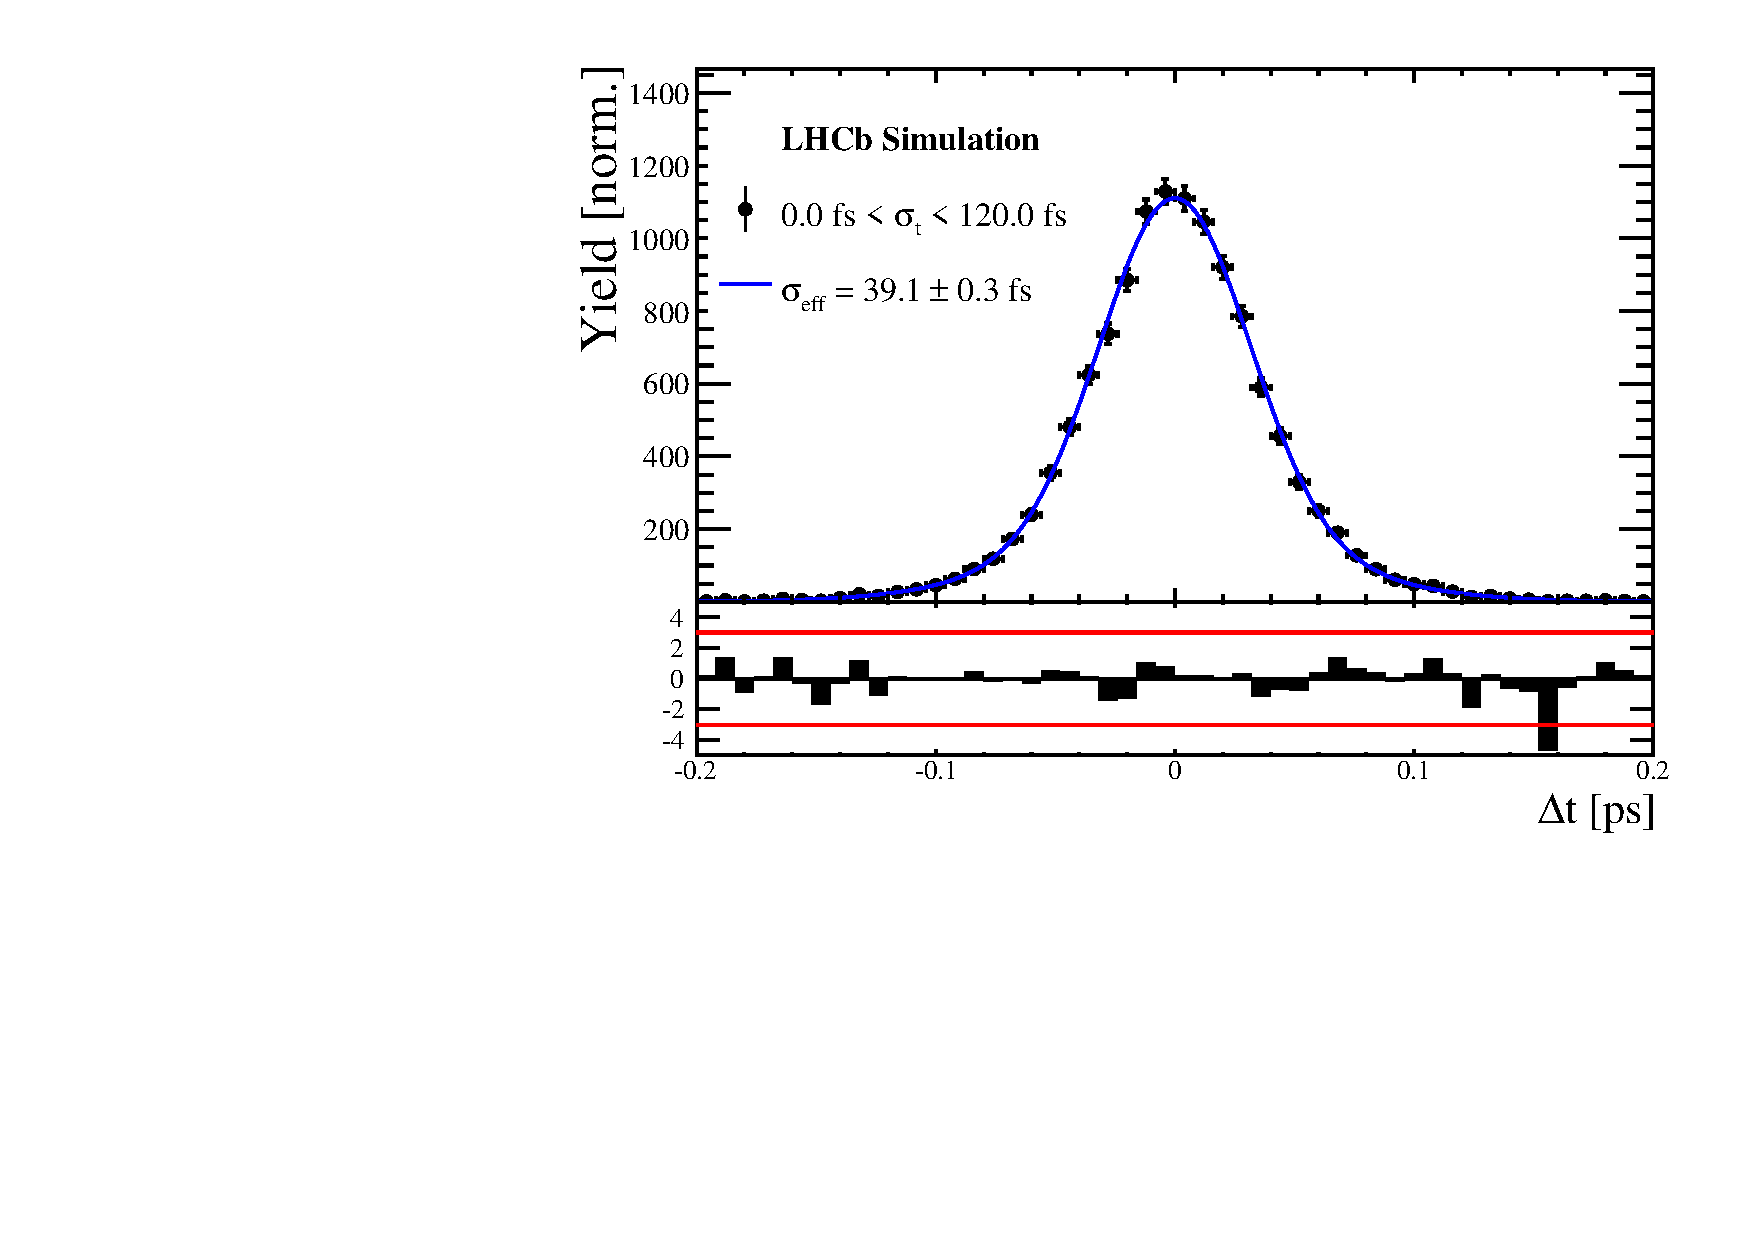
\includegraphics[height=!,width=0.49\textwidth]{figs/Resolution/SignalMC_bin_all.pdf}
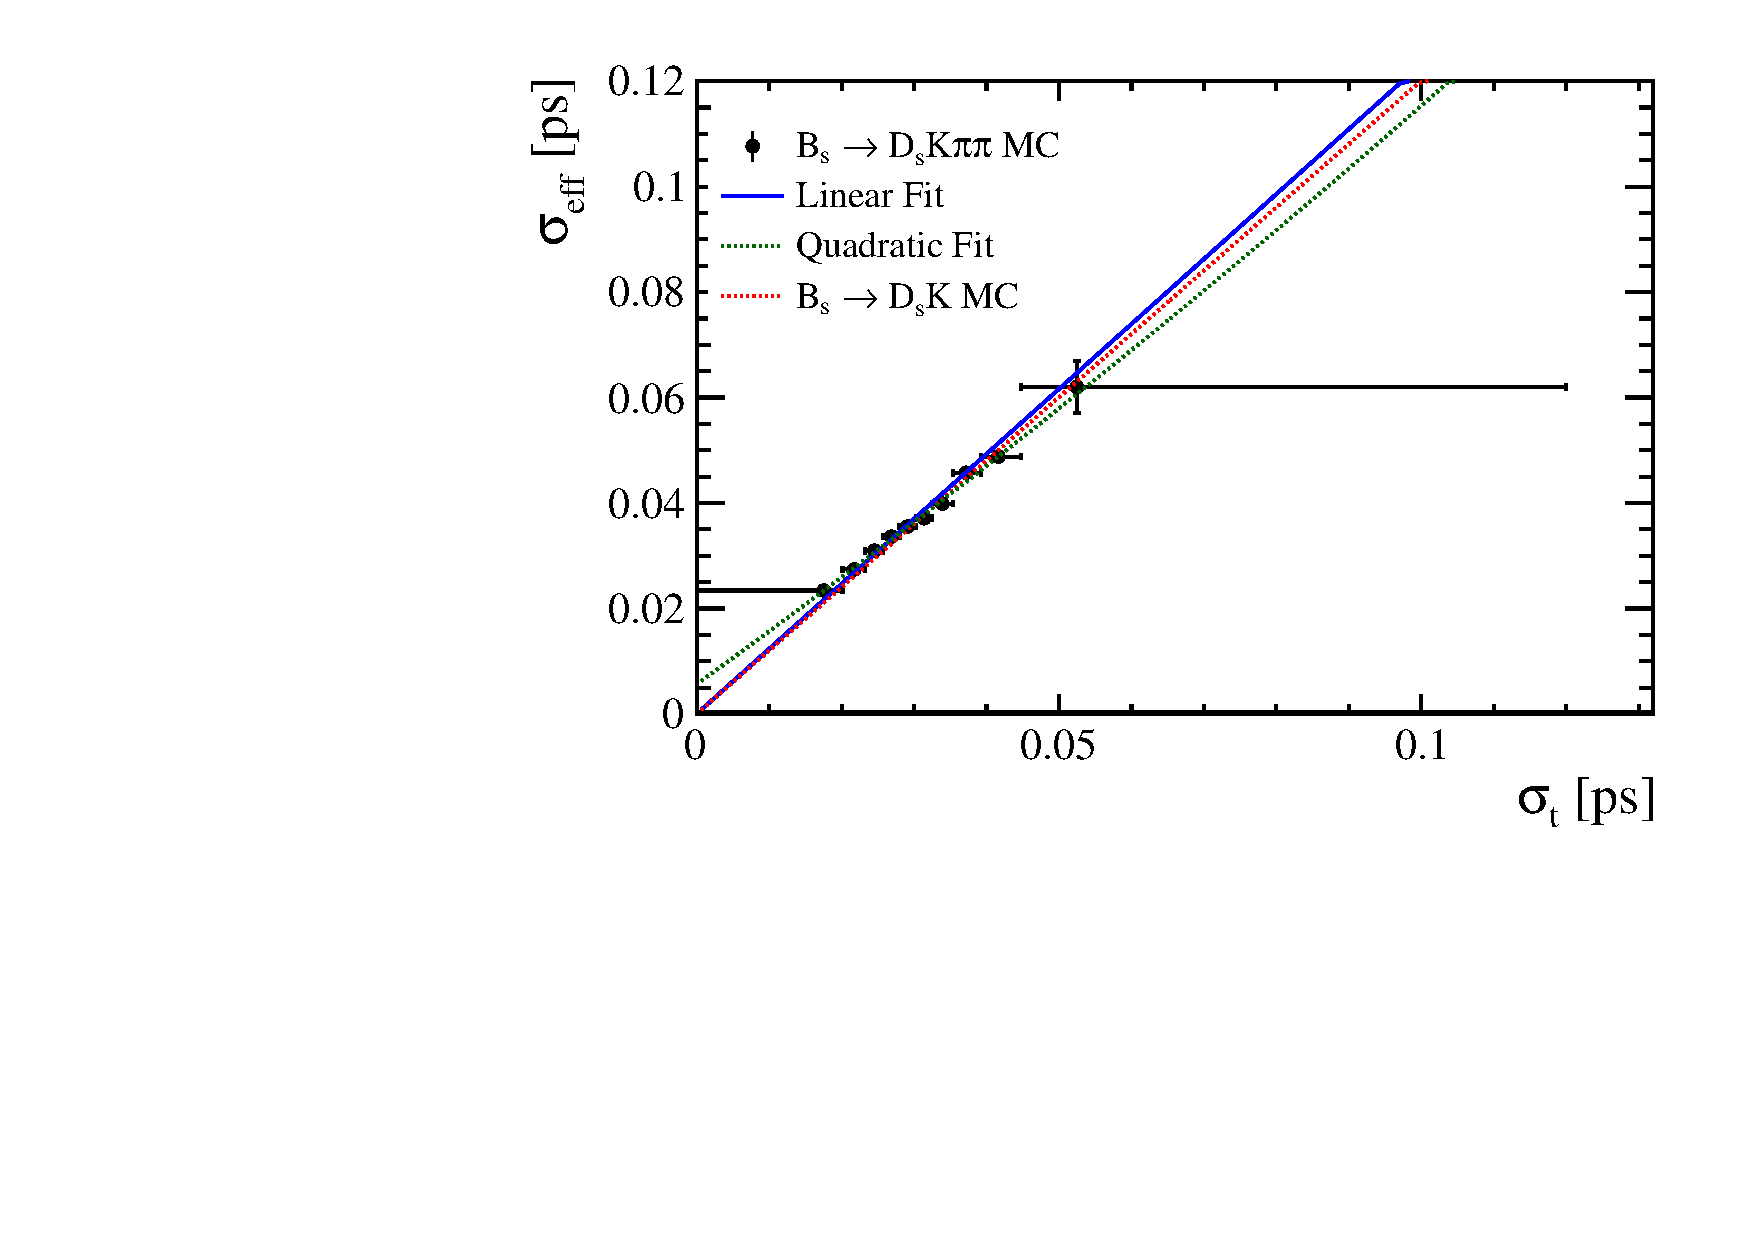
\includegraphics[height=!,width=0.49\textwidth]{figs/Resolution/ScaleFactor_MC.pdf}
\caption{ (Left) Difference of the true and measured decay time of $\Bs\to\Ds\kaon\pion\pion$ MC candidates. 
(Right) The measured resolution $\sigma_{eff}$ as function of the per-event decay time error estimate $\sigma_t$ for $B_s \to D_s K \pi \pi$ MC (Run-I). 
The fitted calibration curve is shown in blue.}
\label{fig:scaleFactorMC}
\end{figure}

%\clearpage
\subsection{Calibration for Run-II data }

For the resolution calibration of Run-II data, a sample of promptly produced $D_s$ candidates is selected
using the \textsf{B02DsKPiPiLTUBD2HHHBeauty2CharmLine} stripping line.
This lifetime-unbiased stripping line does not apply selection requirements related to lifetime or impact parameter, allowing for a study of the resolution. 
In order to reduce the rate of this sample it is pre-scaled in the stripping.
%The stripping line cuts are summarized in Tab.  
Each $D_s$ candidate is combined with a random kaon track and two random pion tracks which originate from the PV to obtain a sample of fake $B_s$ candidates with a known true decay-time of $t_{true} = 0$. 
The difference of the measured decay time, $t$, of these candidates with respect to the true decay time is attributed to the decay time resolution. 


The offline selection of the fake $B_s$ candidates is summarized in Tab.~\ref{table:fakeBsel}.
The selection is similar than the one for real data with the important difference that the $D_s$ candidate is required to come from the PV by cutting on the impact parameter significance.
Even after the full selection, a significant number of multiple candidates is observed.
These are predominantly fake $B_s$ candidates that share the same $D_s$ candidate combined with different random tracks from the PV.
We select one of these multiple candidates randomly which retains approximately $20\%$ of the total candidates.
The invariant mass distribution of the selected $D_s$ candidates is shown in Fig.~\ref{fig:ResoFit_Ds}.
To separate true $D_s$ candidates from random combinations, the \textsf{sPlot} method is used to statistically subtract combinatorial background from the sample.

Figure \ref{fig:scaleFactorData} shows the \textsf{sWeighted} decay-time distribution for fake $B_s$ candidates.
Similar as in the previous section, the decay-time distribution is fitted with a double-Gaussian resolution model in slices of the per-event decay time error.
Since some $D_s$ candidates might actually originate from true $B_s$ decays, the decay-time distribution of the fake $B_s$ candidates 
might show a bias towards positive decay times. 
Therefore, we determine the decay-time resolution from the negative decay-time distribution only.
Details of the fit results in each slice are shown in appendix \ref{sec:DecResFits}. 
The resulting calibration function:
\input{tables/Resolution/ScaleFactor_Data.txt}
is in good agreement with the one obtained for the $B_s \to J/\psi \phi$ (Run-II) analysis. 
\begin{equation}
\sigma_{eff}^{J/\psi\phi}(\sigma_t) = \left( 12.25 \pm 0.33 \right) \text{fs} + \left( 0.8721 \pm 0.0080 \right) \sigma_t
\label{eq:scaleFactorJpsiPhi}
\end{equation}

%\clearpage
\begin{table}[h]
\centering
\caption{Offline selection requirements for fake $B_s$ candidates from promptly produced $D_s$ candidates combined with random prompt $K\pi\pi$ bachelor tracks.}
%\resizebox{\linewidth}{!}{
 \renewcommand{\arraystretch}{1.0}
 \small
 \begin{tabular}{l l l}
\hline
\hline
 & Description & Requirement  \\
\hline
$B_s \to D_s K \pi \pi$  &  $\chi^{2}_{vtx}/\text{ndof}  $&$ <  8$ \\
&  $\chi^{2}_{DTF}/\text{ndof} $&$   <  15 $ \\
& $t$  & $< 0 \ps$ \\
\\
$D_s \to h h h$ &  $\chi^{2}_{vtx}/\text{ndof}  $&$ <  5$  \\
& DIRA &$ > 0.99994$ \\
& $\chi^{2}_{FD}$ & $> 9$ \\
& $p_T$ & $> 1800$ MeV \\
& $\chi^{2}_{IP}$ & $< 9$ \\
&  $\chi^{2}_{IP}(h)$ &  $> 5$ \\
& Wrong PV veto & nPV = 1 $||$  $\text{min}(\Delta\chi^{2}_{IP}) > 20$ \\
\\
$D_s^- \to K K \pi^-$  & $D^0$ veto  & $m(K K) < 1840$ MeV \\
& $D^-$ veto  & $m(\Kp K^-_\pi \pim) \ne m(D^-) \pm 30$ MeV \\
& $\Lambda_c$ veto  & $m(\Kp K^-_p \pim) \ne m(\Lambda_c) \pm 30$ MeV \\
\\
$D_s^- \to \phi \pi^-$ & $m(KK)$  & $= m_{\phi} \pm 20$ MeV \\
& PIDK($K^+$) & $> -10$ \\
& PIDK($K^-$) & $> -10$ \\
& PIDK($\pi^-$) & $< 20$ \\
\\
$D_s^- \to K^{*}(892) K^-$ & $m(KK)$  & $\ne m_{\phi} \pm 20$ MeV \\
& $m(K^+\pi^-)$  & $= m_{K^{*}(892)} \pm 75$ MeV \\
& PIDK($K^+$) & $> -10$ \\
& PIDK($K^-$) & $> -5$ \\
& PIDK($\pi^-$) & $< 20$ \\
\\
$D_s^- \to (K K \pi^-)_{NR}$ & $m(KK)$  & $\ne m_{\phi} \pm 20$ MeV \\
& $m(K^+\pi^-)$  & $\ne m_{K^{*}(892)} \pm 75$ MeV \\
& PIDK($K^+$) & $> 5$ \\
& PIDK($K^-$) & $> 5$ \\
& PIDK($\pi^-$) & $< 10$ \\
\\
$D_s \to \pi \pi \pi$ & PIDK($h$) & $< 10$  \\
& PIDp($h$) & $< 10$ \\
& $D^0$ veto  & $m(\pip \pim) < 1700$ MeV \\
\\
$X_s \to K \pi \pi$  &  $\chi^{2}_{IP}(h)$ &  $< 40$ \\
& PIDK(K) & $> 10$ \\
& PIDK($\pi$) & $< 5$ \\
& isMuon($h$) & False \\
\\
All tracks  & $p_T$ & $> 500$ MeV \\

\hline
\hline
\end{tabular}
%}
\label{table:fakeBsel}
\end{table}
%\clearpage

\begin{figure}[h]
\centering
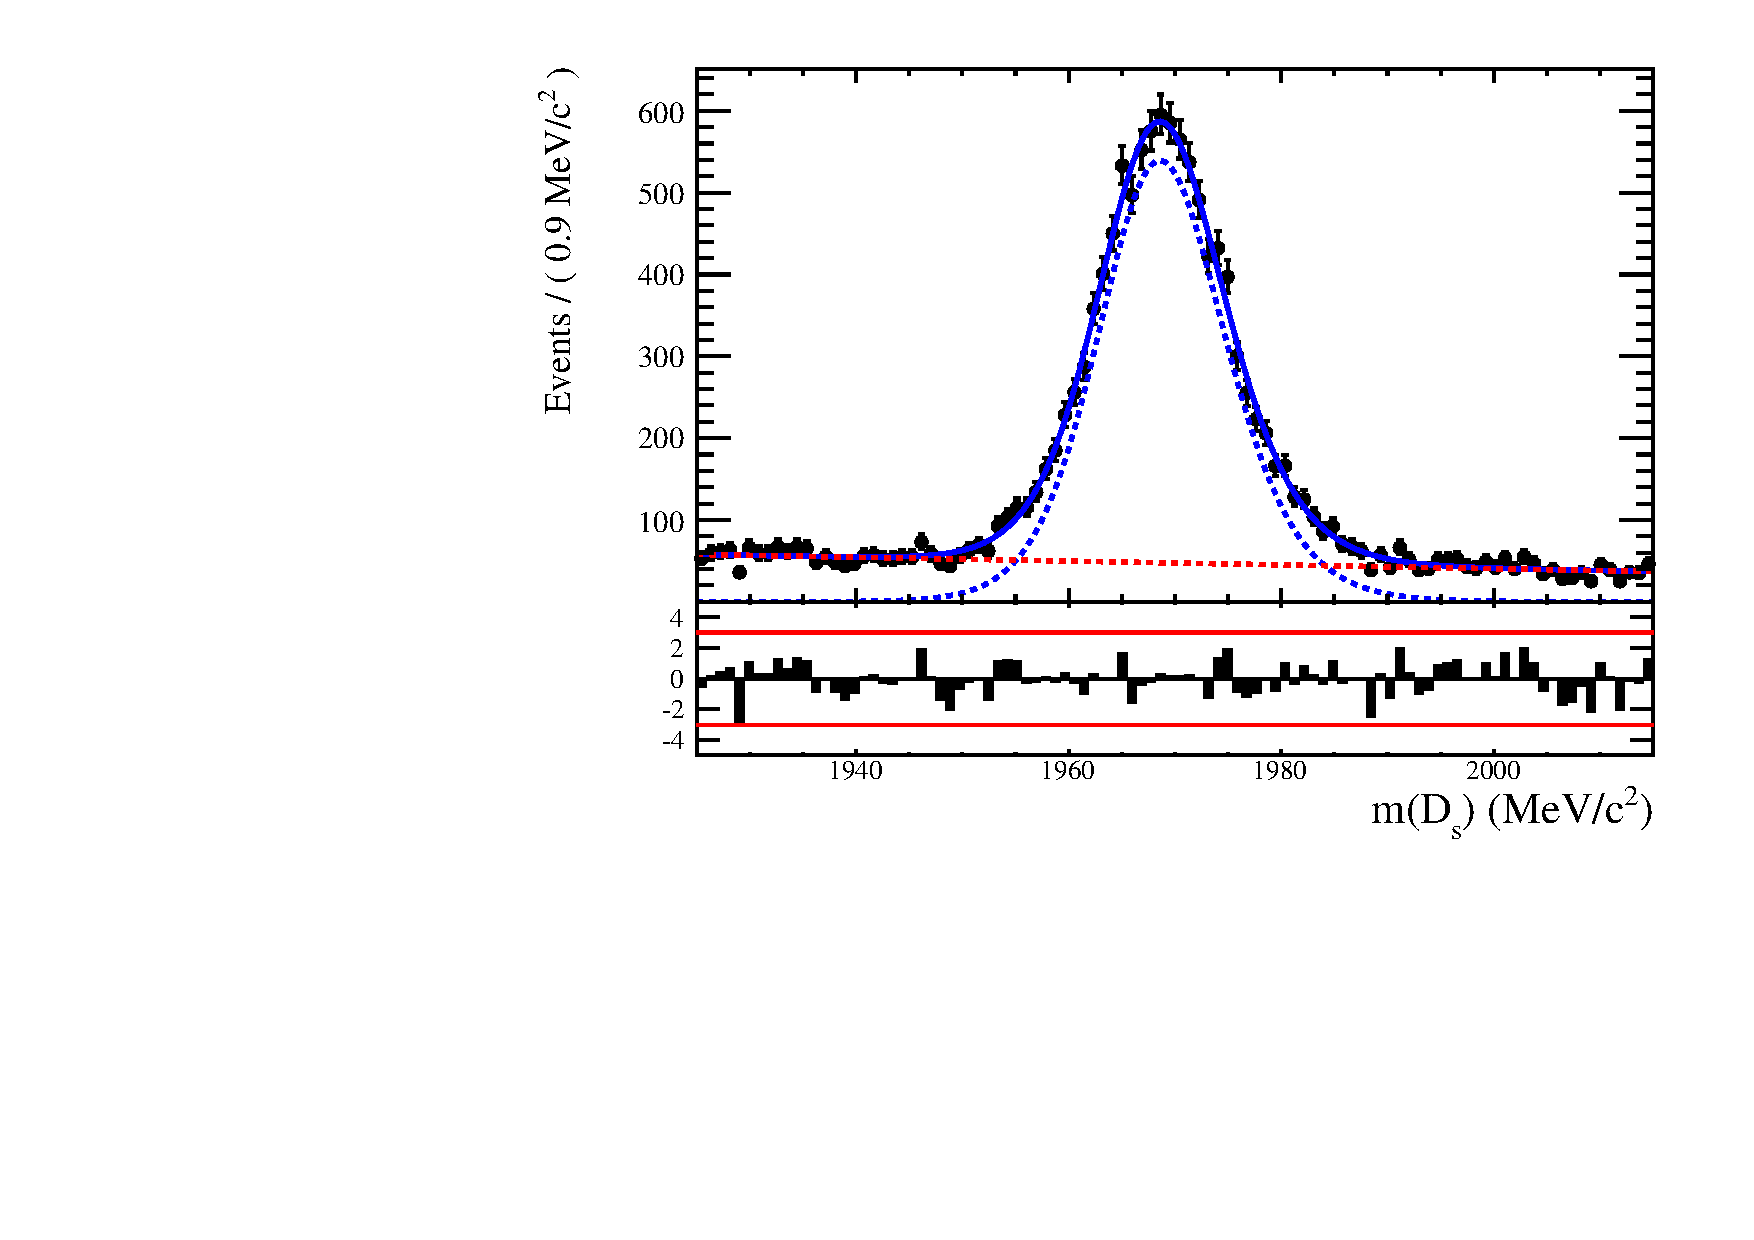
\includegraphics[height=!,width=0.49\textwidth]{figs/Resolution/Ds_M_pull.pdf}
\caption{The invariant mass distribution for prompt $D_s$ candidates. }
\label{fig:ResoFit_Ds}
\end{figure}

\begin{figure}[h]
\centering
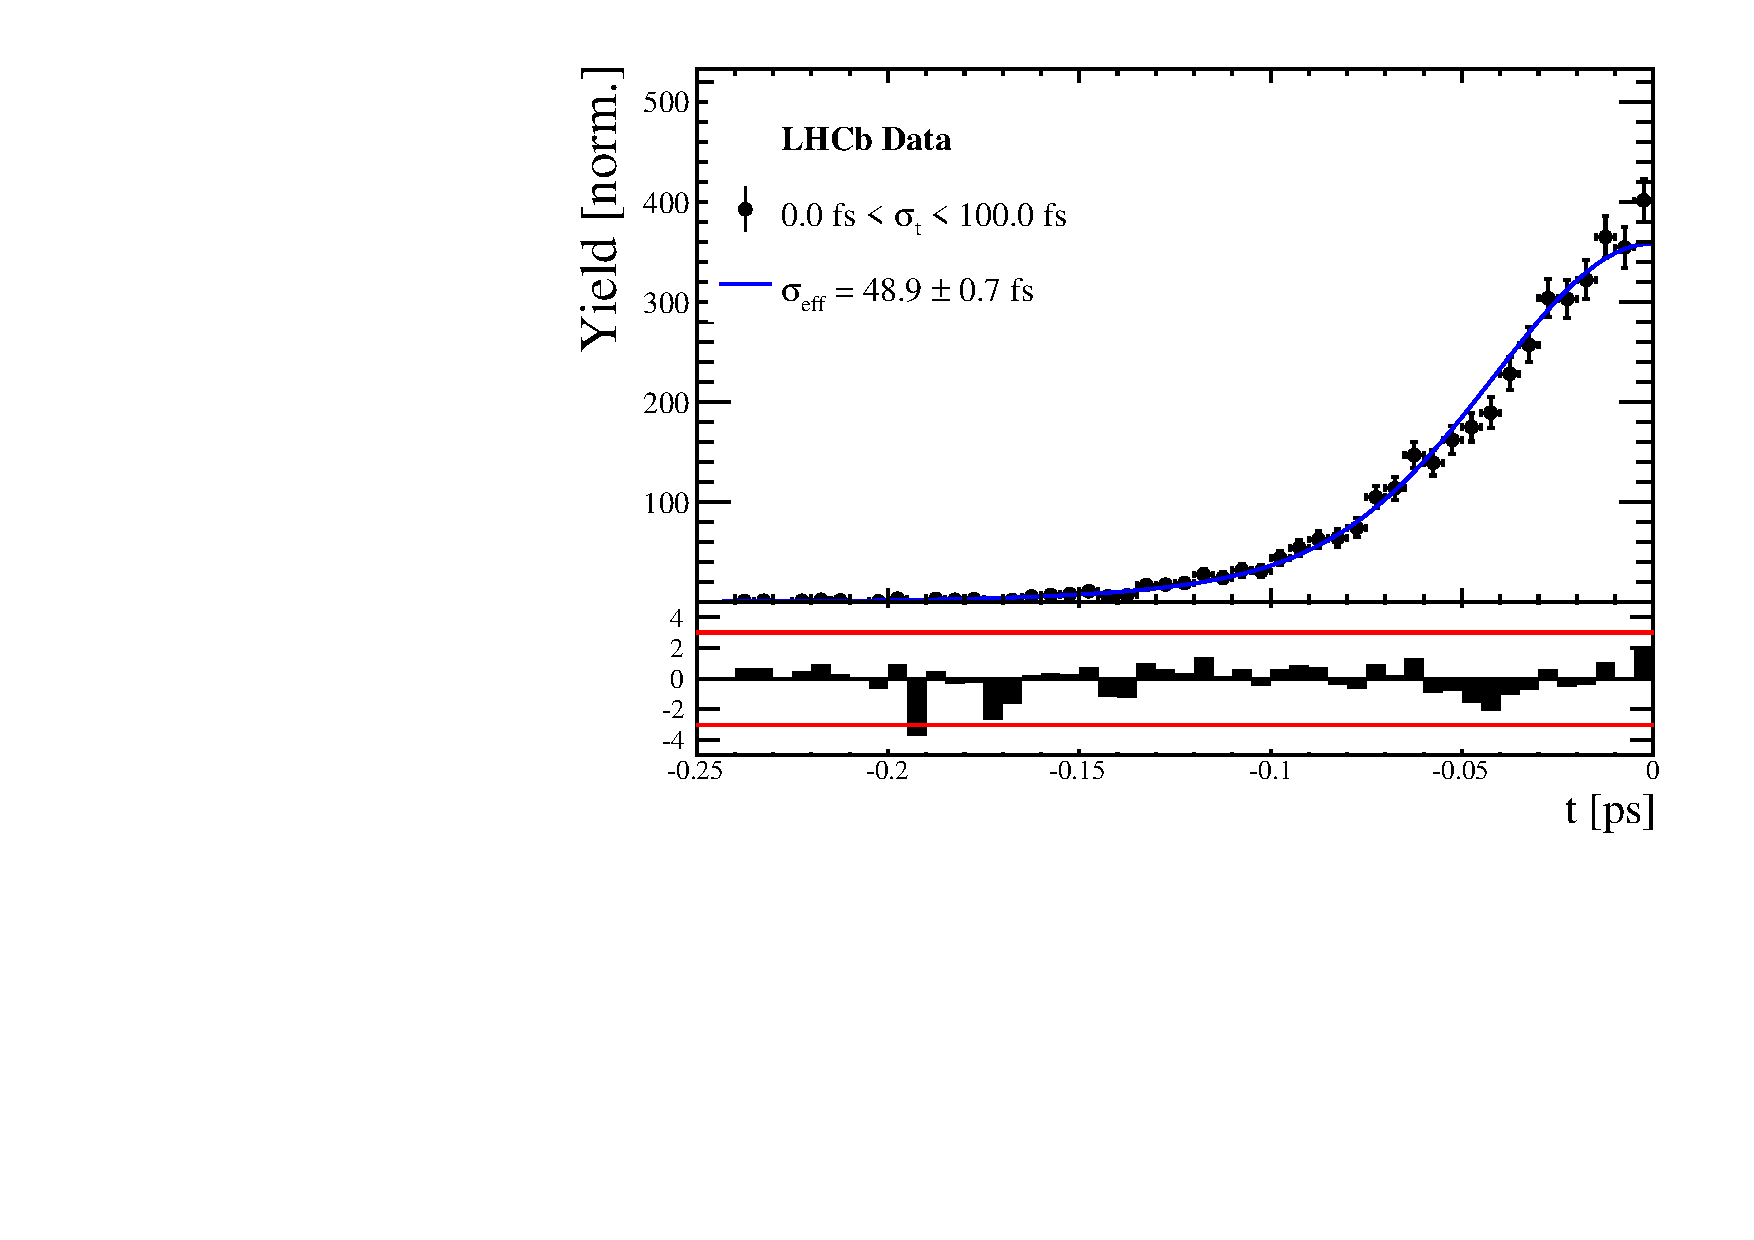
\includegraphics[height=!,width=0.49\textwidth]{figs/Resolution/SignalData_bin_all.pdf}
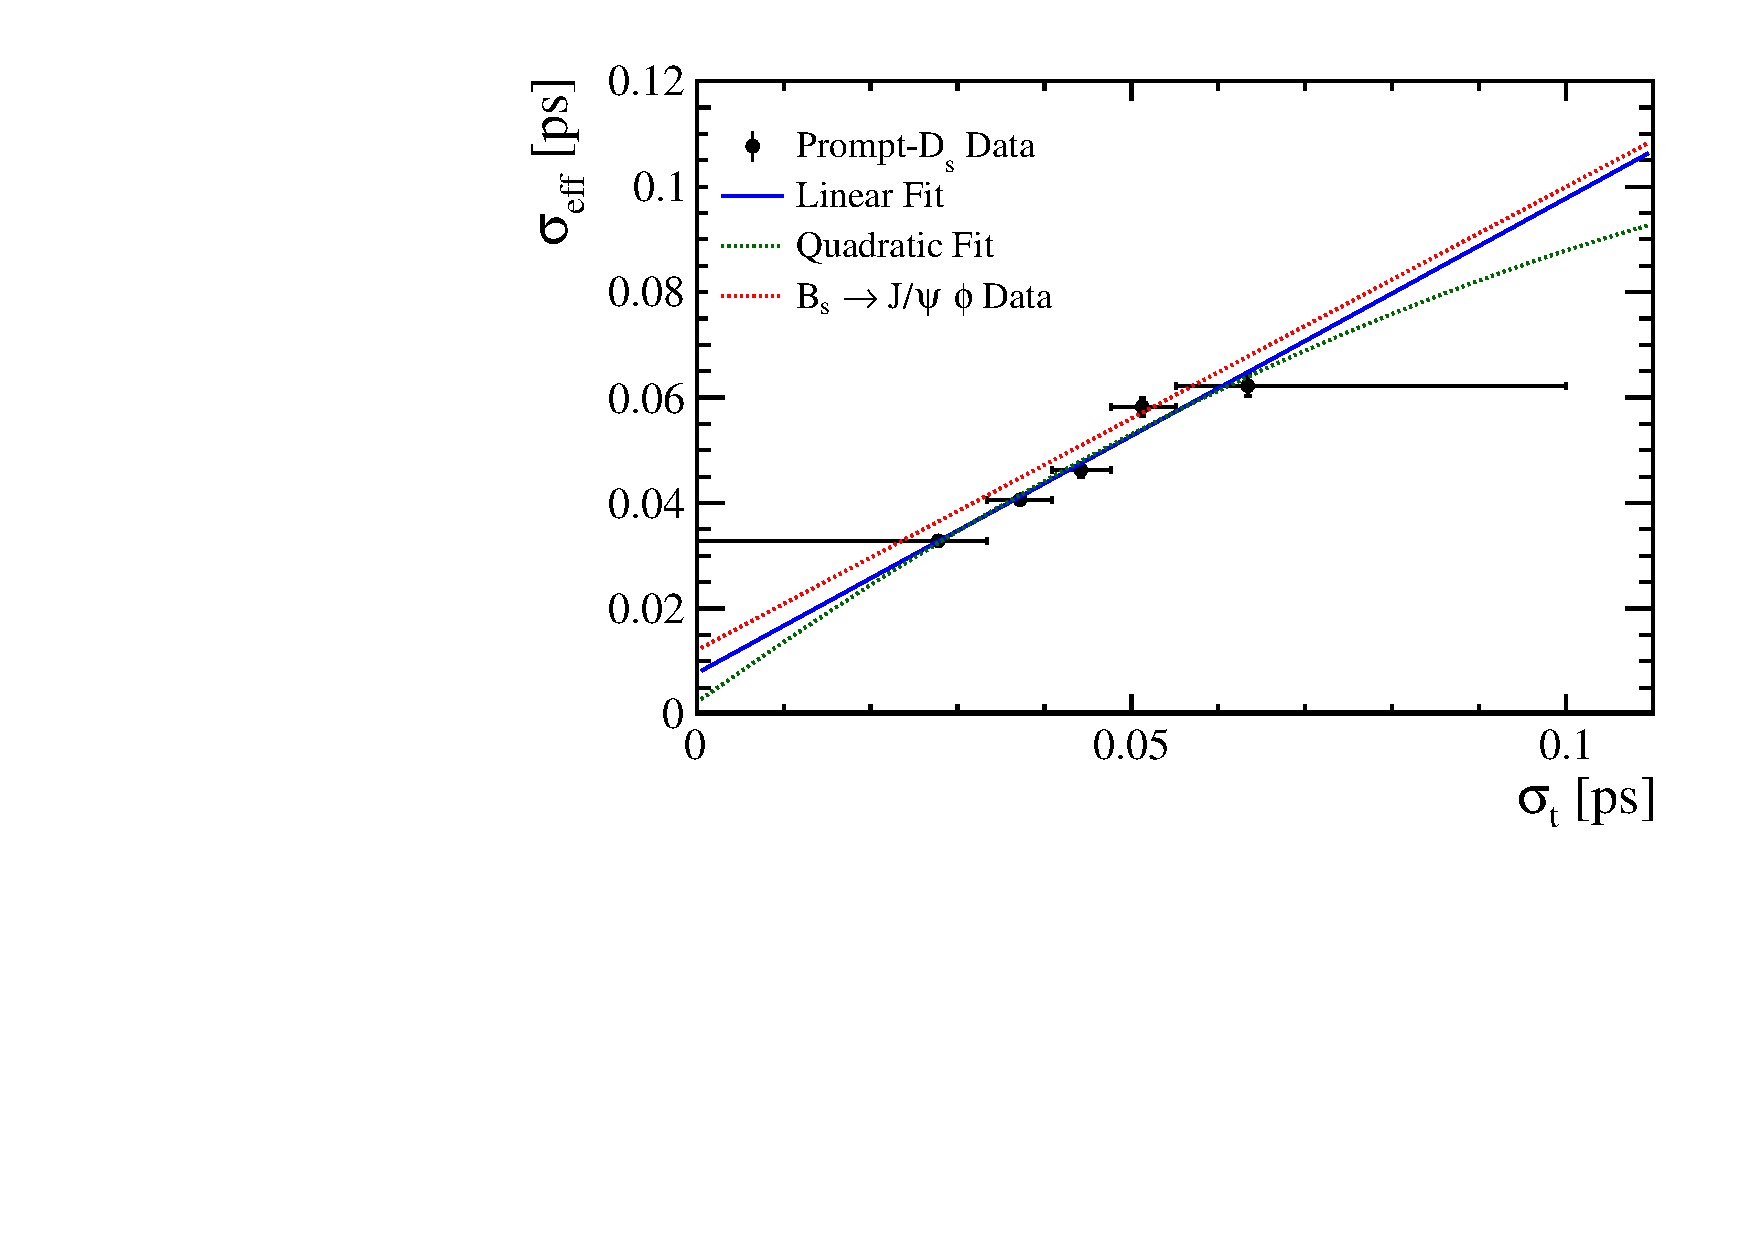
\includegraphics[height=!,width=0.49\textwidth]{figs/Resolution/ScaleFactor_Data.pdf}
\caption{ (Left) Decay-time distribution for fake $B_s$ candidates from promptly produced $D_s$ candidates, combined with random prompt $K\pi\pi$ bachelor tracks.
(Right) The measured resolution $\sigma_{eff}$ as function of the per-event decay time error estimate $\sigma_t$ for fake $B_s$ candidates (Run-II data).
The fitted calibration curve is shown in blue.}
\label{fig:scaleFactorData}
\end{figure}


\clearpage
\subsection{Cross-checks}

\subsubsection{Kinematic dependence}

\begin{figure}[h]
\centering
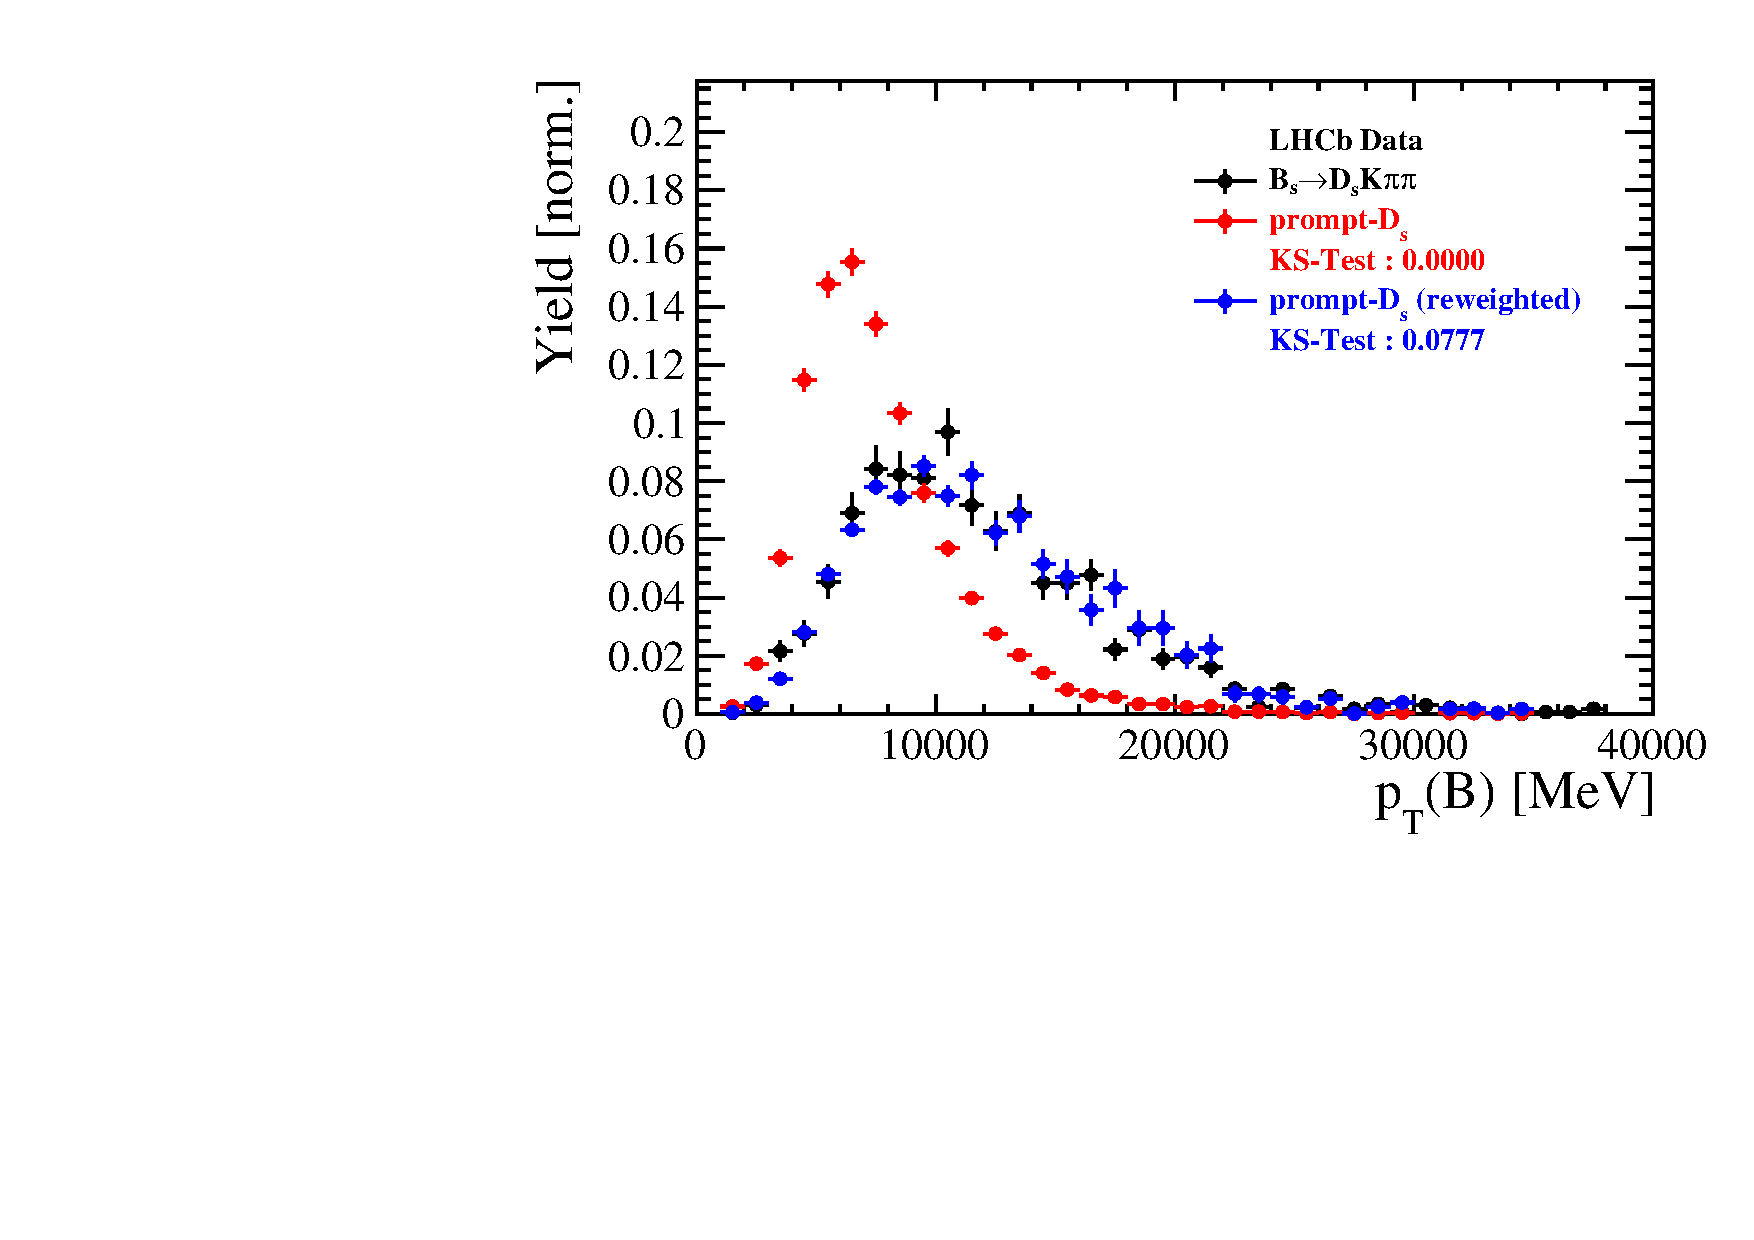
\includegraphics[height=!,width=0.3\textwidth]{figs/dataVsMC/LTU/combined/Ds2all_2_Bs_PT.pdf}
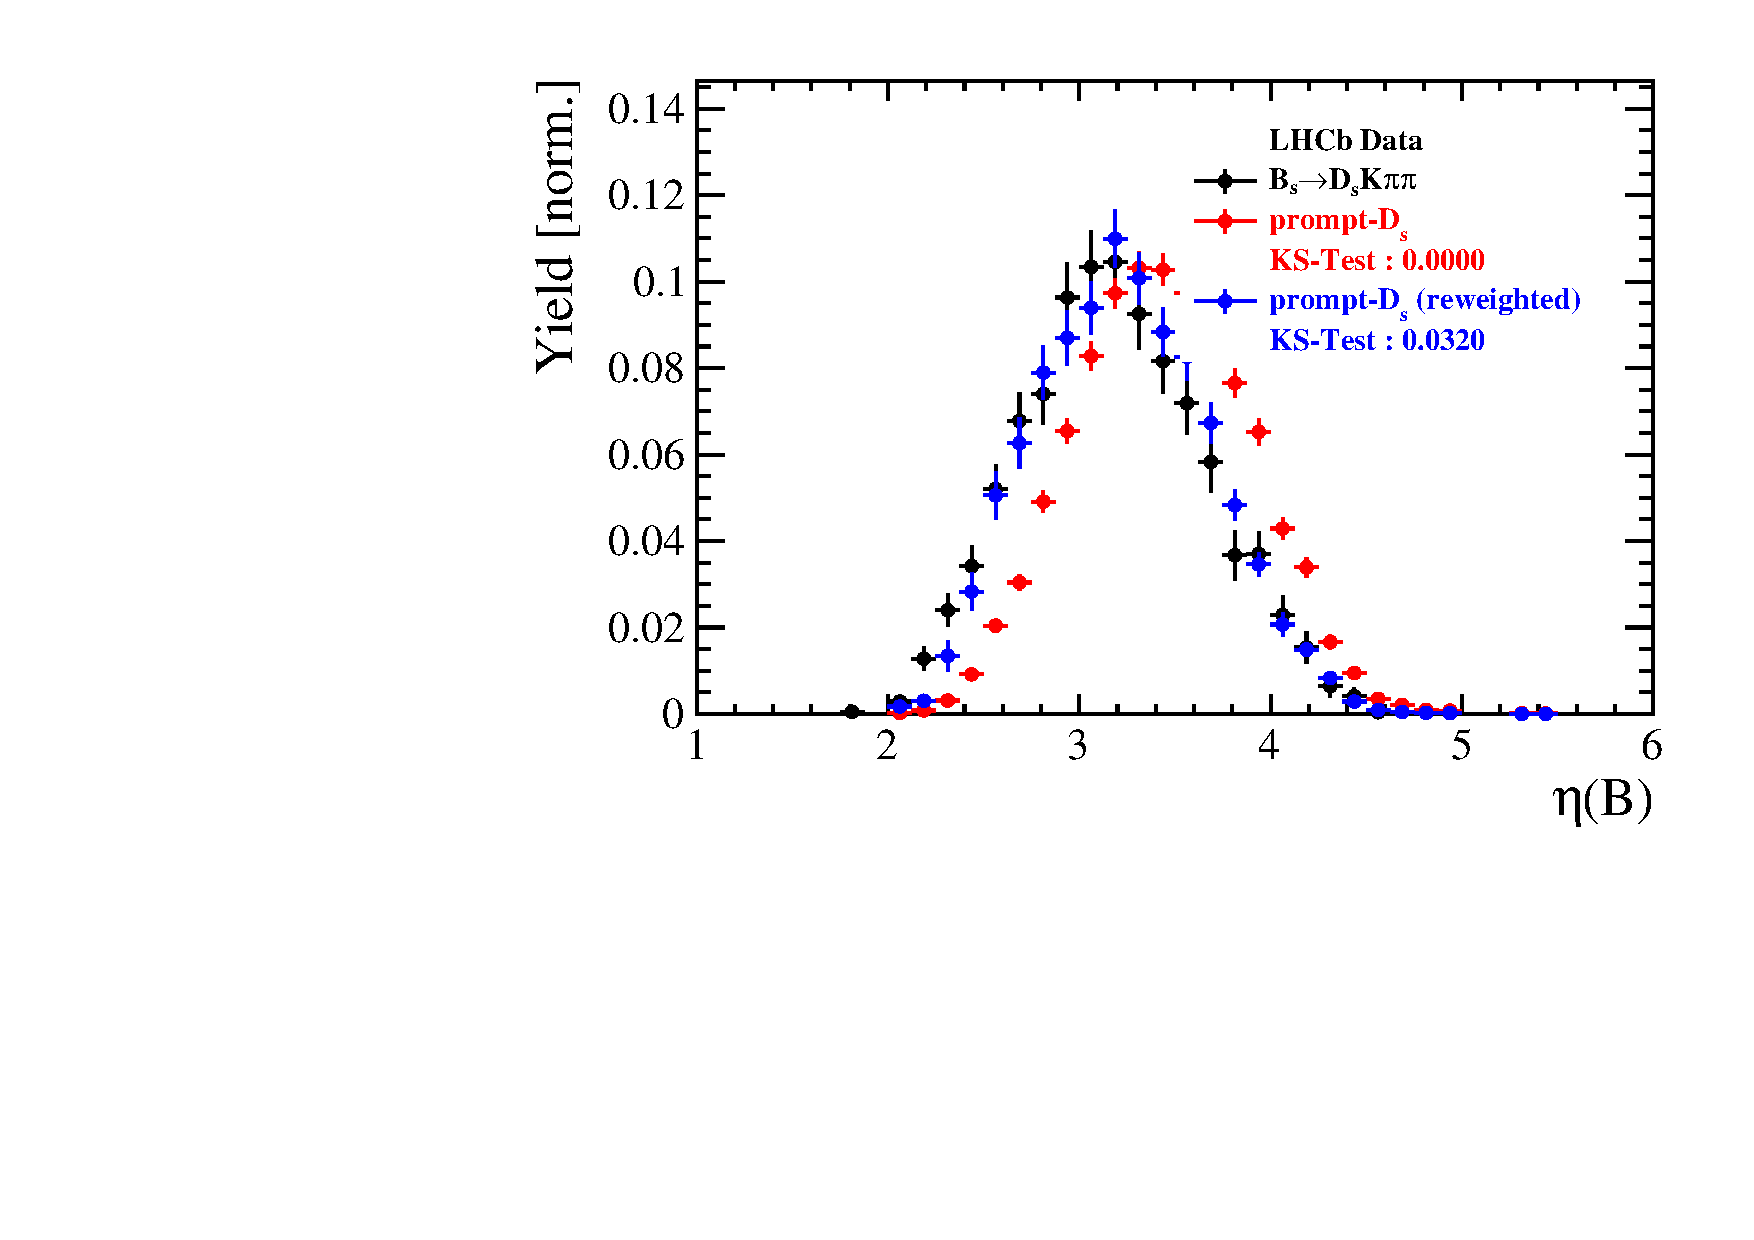
\includegraphics[height=!,width=0.3\textwidth]{figs/dataVsMC/LTU/combined/Ds2all_2_Bs_ETA.pdf}
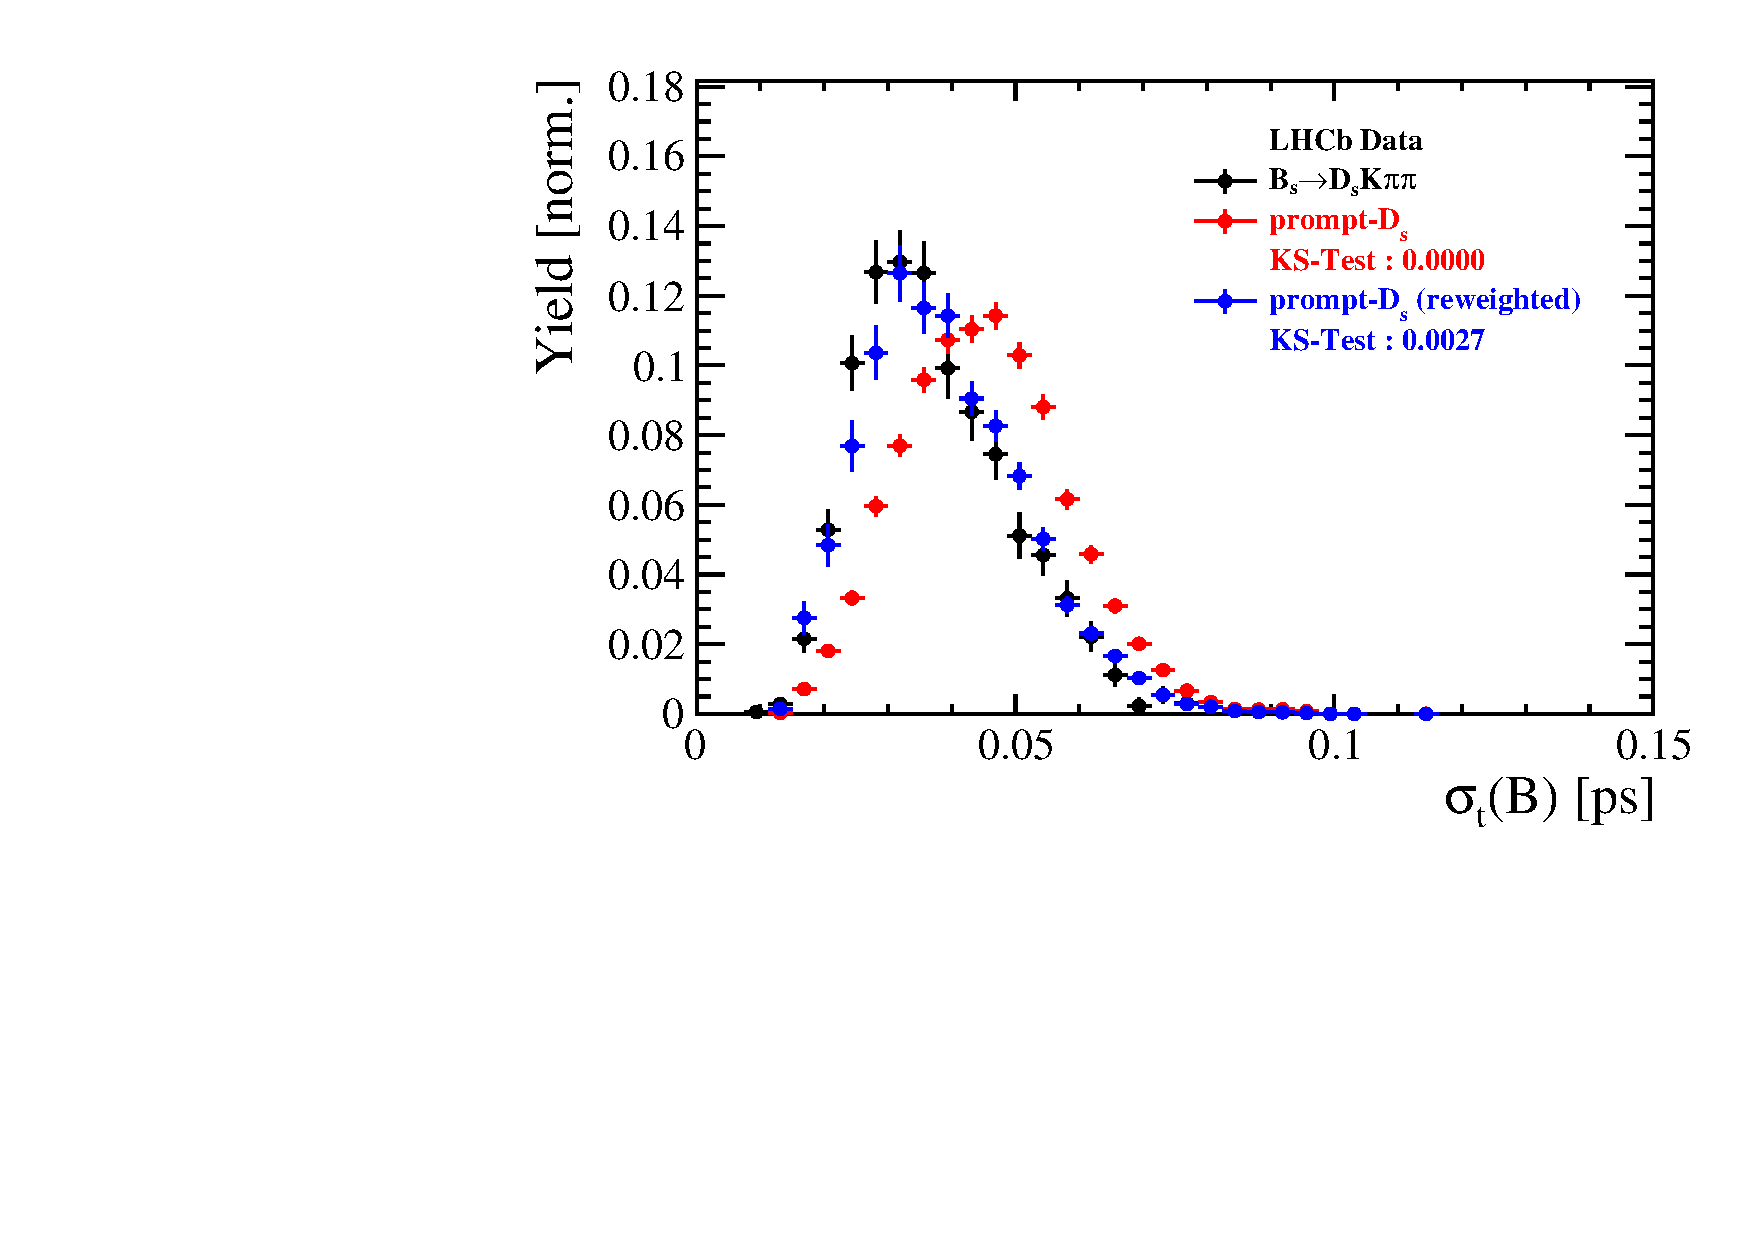
\includegraphics[height=!,width=0.3\textwidth]{figs/dataVsMC/LTU/combined/Ds2all_2_Bs_DTF_TAUERR.pdf}
\caption{}
\label{fig:}
\end{figure}

\subsubsection{DTF constraints}
